\chapter{Alcances de la memoria}
\label{alcansces}

\section{Problema a resolver}

Actualmente Chile no cuenta con grandes plantas de energía solar fotovoltaica y este proyecto será uno de los primeros para el bombeo de agua mediante el uso de la energía solar para una empresa exportadora de frutas con lo cual se convertirá en un proyecto modelo para próximos proyectos.\\

La difusión de la información de producción permitirá a los miembros de la RedSolLac contar con información para el desarrollo de estudios y proyectos en Chile y toda la región.\\

El sistema informático actual recibe la información de los inversores y su sistema de medición de energía y almacenamiento de datos, los envía a un sistema privado el cual no permite la publicación y uso de la información por lo que es necesario implementar un sistema que permita publicar dichos datos.\\

\begin{figure}[h!]
        \centering
        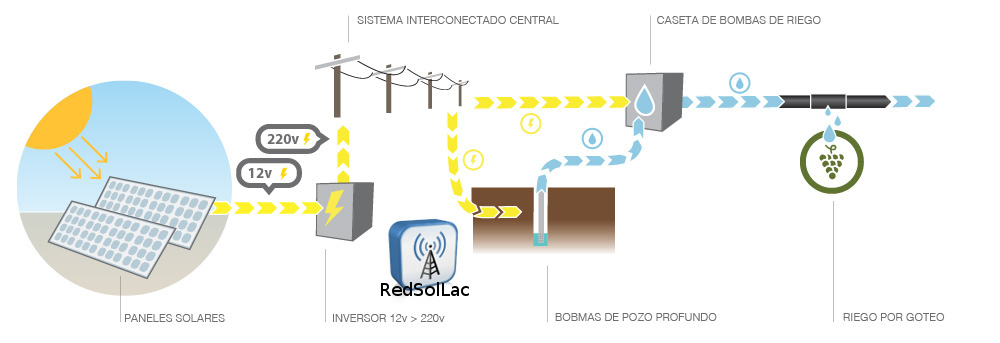
\includegraphics[scale=0.4]{images/plantaSubSoleEsquema}
        \caption{\tiny Esquema planta fotovoltaica Subsole 307,2 kWp(STC) a la red eléctrica EMELAT - Región de Atacama}
\end{figure}

La planta eléctrica de Subsole, descrita en la figura de arriba, tiene como objetivo producir suficiente energía que le permita alimentar los motores que extraen el agua de los posos destinados al riego por goteo, sin embargo la energía eléctrica producida por la planta no va directamente al sistema eléctrico de los posos, si no que esta se vende al sistema interconectado central actuando como un productor de energía, luego los motores de los posos usan energía del SIC como cualquier consumidor de electricidad. Los inversores que figuran en el esquema permiten convertir la electricidad producida por los paneles a corriente alterna y 220 Volt, adicionalmente los inversores tienen la capacidad de registrar toda la información de potencia que pasa por ellos. Dentro del trabajo realizado en esta memoria se contempla instalar un sistema de comunicación para los inversores que permitan enviar la información directamente a una base de datos de la RedSolLac en internet.

Los principales actores y usuarios a los que este sistema dará acceso a dicha información serán todos los miembros de la RedSolLac\cite{redSolLac:1}, interesados en recibir y compartir información relacionada con la energía solar fotovoltaica. La plataforma será abierta por lo que cualquier otro usuario podrá acceder a esta información.\\

El BID a través de este proyecto que desarrolla la Fundación Chile espera conectar a través de esta red a los actores claves en el desarrollo de proyectos fotovoltaicos de Latinoamérica y el Caribe. En la actualidad, existen pocos proyectos en la región por lo que el conocimiento técnico en esta materia en la región se reduce a experiencias de universidades y algunas iniciativas privadas aisladas. La información generada por la planta fotovoltaica Subsole será un sitio de referencia para el estudio y desarrollo de nuevas plantas.\\

\begin{figure}[h!]
        \centering
        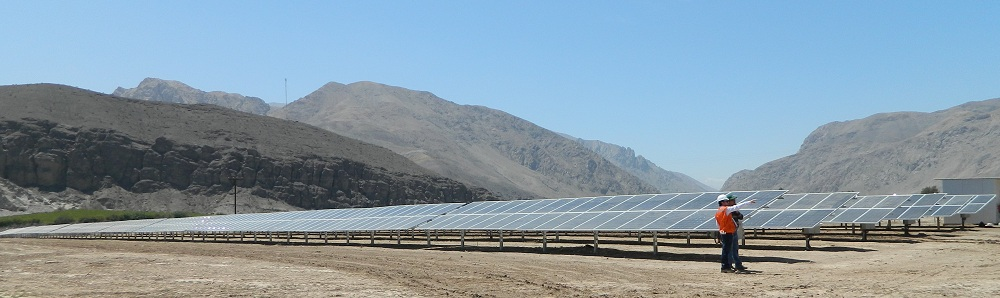
\includegraphics[scale=1.4]{images/plantaSubSoleLorosAmarilla}
        \caption{\tiny Planta fotovoltaica 307,2 kWp, sector Los Loros - Tierra Amarilla, región de Atacama - Chile}
\end{figure}

La estación de medición de radiación solar, temperatura y humedad ambiente instalada en Fundación Chile, Av. Parque Antonio Rabat 6165, Vitacura, Santiago de Chile, en conjunto con la estación meteorológica de la planta fotovoltaica, proporcionarán la información de radiación solar para la calculadora fotovoltaica. Se espera en el futuro incorporar más estaciones de medición.\\

\begin{figure}[h!]
        \centering
        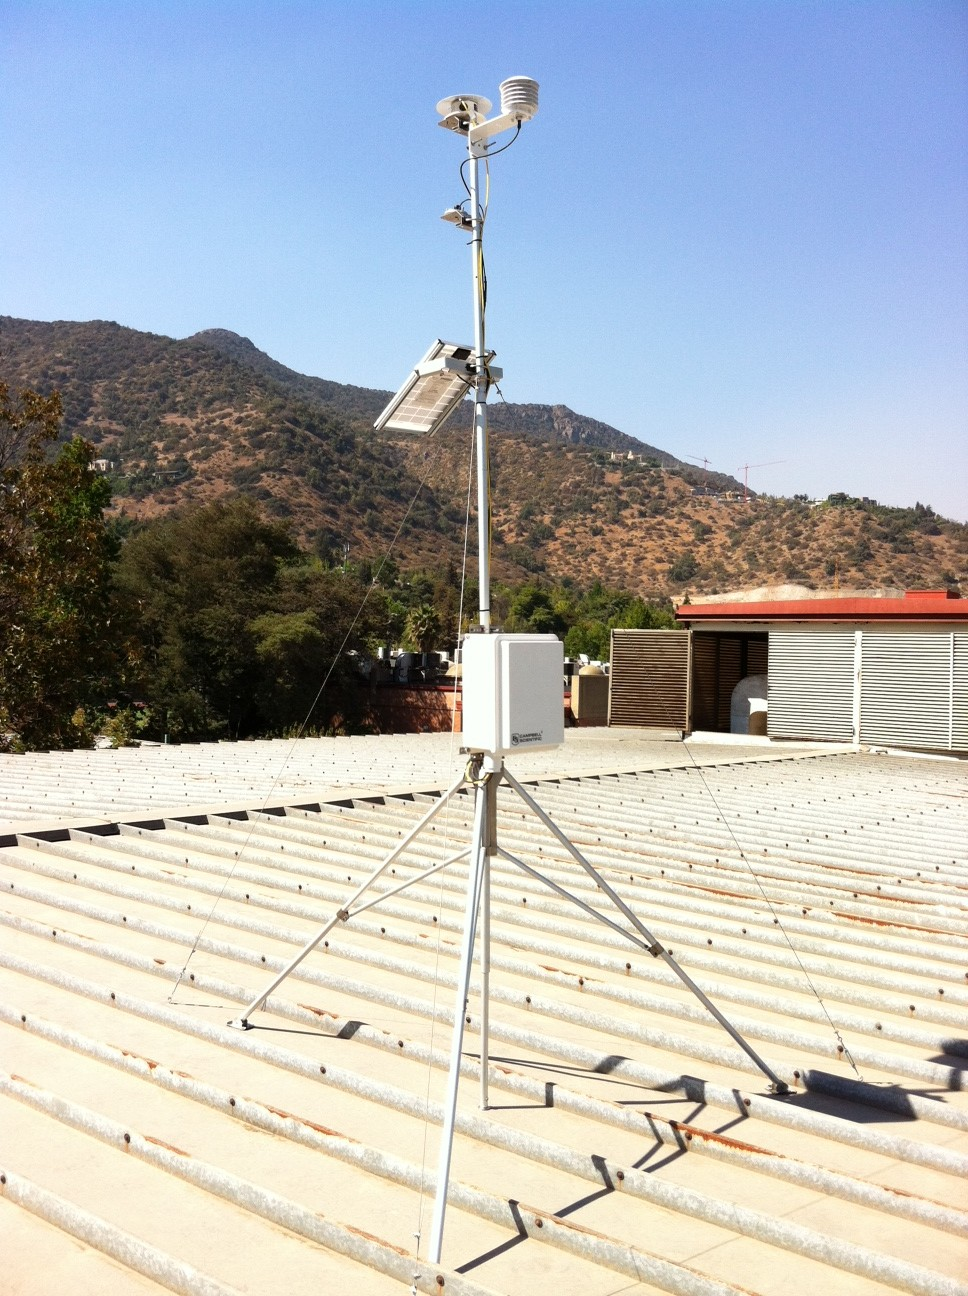
\includegraphics[scale=0.12]{images/estacionMedicionFch}
        \caption{\tiny Estación de medición de radiación solar en Fundación Chile, Vitacura - Santiago.}
\end{figure}

El desarrollo de esta memoria permitirá la comunidad de la RedSolLac contar con una gran base de datos para ofrecer a todos sus usuarios, así como diversas aplicaciones en su plataforma para la defunción y el patrocinio de la utilización de energía solar en la región. Una red como esta potenciara el desarrollo de todas las energías renovables no convencionales(ERNC) especialmente la solar fotovoltaica lo cual atraerá un beneficio medioambiental para toda la comunidad tanto pertenecientes a la red como a la población en general.

\section{Objetivo principal de la solución}
Desarrollo e implementación de un sistema informático para la Red de energía solar fotovoltaica de Latinoamérica y el Caribe (RedSolLAC) que permita interconectar equipos y estaciones de medición solar para la recolección y explotación de datos e información técnica provenientes de una planta solar ubicada en la región de Atacama, Chile.

\section{Objetivos específicos de la solución}
\begin{itemize}
\item Interconectar los diferentes sistemas que componen las estaciones de medición para que exista una comunicación efectiva entre dichos sistemas y una base de datos común en Internet.
\item Desarrollo de un sistema Web capaz de procesar y publicar la información recopilada de una planta de energía solar de gran potencia, ubicada en la región de Atacama.
\item Desarrollo de una calculadora online para sistemas fotovoltaicos.
\item Realizar pruebas de la plataforma en conjunto con todos sus componentes, comparar los datos obtenidos con datos recopilados manualmente.
\end{itemize}

\begin{figure}[h!]
        \centering
        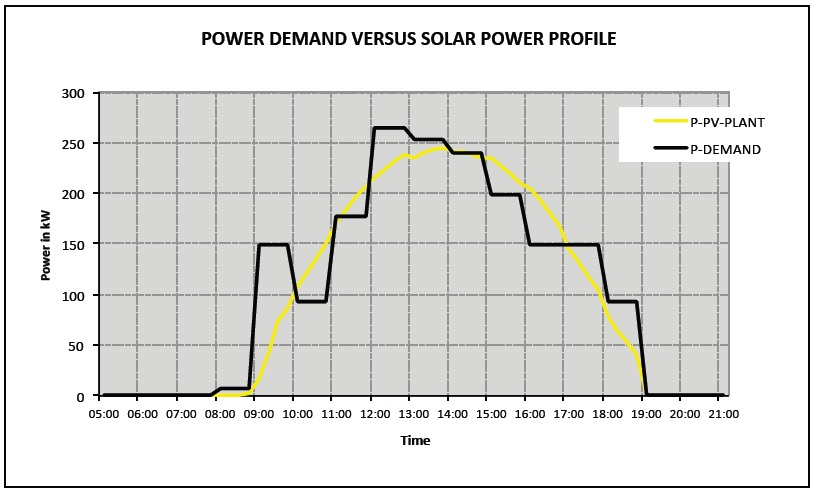
\includegraphics[scale=0.5]{images/demandaGeneracionSubSole}
        \caption{\tiny Gráfico de ejemplo de la curva de demanda de energía versus la generación de energía solar fotovoltaica en la planta Subsole.}
\end{figure}

